\documentclass{beamer}

\usetheme{Madrid}
\usecolortheme{default} % or use {default}

% parse tree
\usepackage[nocenter]{qtree}
\usepackage{tree-dvips}
\usepackage{amsmath}

\title[]{Semantic Parsing Methods}
\subtitle{An Overview}
\author {Xiang Zhang}
%\institute {
%    NLPR\\
%    Institute of Automation
%}
\date{2016.08}
%\logo{\includegraphics[height=1.5cm]{lion-logo.png}}

%------------------------------------------------------------
\AtBeginSection {
    \begin{frame}
        \frametitle{Agenda}
        \tableofcontents[sectionstyle=show/shaded,subsectionstyle=hide/hide/hide]
    \end{frame}
}
\AtBeginSubsection {
    \begin{frame}
        \frametitle{Agenda}
        
        % current subsection / other subsections of current section / other subsections
        \tableofcontents[subsectionstyle=show/shaded/hide]
    \end{frame}
}
%------------------------------------------------------------

\begin{document}

\frame{\titlepage}

%---------------------------------------------------------
%This block of code is for the table of contents after
%the title page
\begin{frame}
\frametitle{Agenda}
\tableofcontents[hideallsubsections]
\end{frame}
%---------------------------------------------------------


\section{Semantics}

\begin{frame}
    \frametitle{Background}

    When it comes to the understanding of natural language sentences, NLP researchers 
    solve it in various granularities.

    These tasks differ in the amount of information they use.

    \begin{itemize}
        \item <1-> Information Extraction (less informative) \\
            \begin{center}
                \emph{is\_a(Obama, PRESIDENT)}
            \end{center}

        \item <2-> Summarization (modestly informative) \\
            \begin{center}
            \emph{Obama wins.}
            \end{center}

        \item <3-> Semantic Parsing (exact matching) \\
            \begin{center}
            $\exists e . beat(e) \wedge Sub(e, Obama) \wedge Obj(e, Romney)$
            \end{center}
            
    \end{itemize}

    \uncover<4->{\begin{block}{Caveat}
        \emph{Semantic} here is more of \emph{composition} than telling apart
        from \emph{word senses}.
    \end{block}}
\end{frame}

\begin{frame}
    \frametitle{Semantic Parsing Task}

    The key task of semantic parsing is to find an $f$ such that

    \[
        f: Sentence \to LogicForm
    \]

    \pause

    Generally, there are 3 aspects a semantic parser need take into consideration:

    \begin{itemize}
        \item Modelling: how to represent a logic form
        \item Parsing: design a grammar and parsing algorithm
        \item Learning: use supervision to fix parameters
    \end{itemize}

\end{frame}


\subsection{Davidsonian Representation}

\begin{frame}
    \frametitle{Logic Form from Example}

    \begin{itemize}

        \item <2->
            Brutus stabs Caesar. \\
            stab(Brutus, Caesar) \structure{predicate}

        \item <3->
            Brutus stabs Caesar with a knife. \\
            stab(Brutus, Caesar, \alert{knife}) \structure{n-ary predicate}

        \item <4->
            Brutus stabs Caesar in the agora. \\
            stab(Brutus, Caesar, \alert{agora}) \structure{ambiguous predicate}

        \item <5->
            Brutus stabs Caesar in the agora with a knife. \\
            stab(Brutus, Caesar) \& \alert{with}(knife) \& \alert{in}(agora)
            \structure{move adjunct apart}

    \end{itemize}

\end{frame}

\begin{frame}
    \frametitle{Logic Form from Example}

    \begin{itemize}
        \item <1-> Brutus stabs Caesar in the agora with a knife. \\
            stab(Brutus, Caesar) \& with(knife) \& in(agora)

        \item <2-> Brutus stabs Caesar with a knife in the agora and twisted it hard. \\
            stab(Brutus, Caesar) \& with(knife) \& in(agora) \& twist(Brutus, knife) \& hard

    \end{itemize}

    \uncover <3-> {
        The standard predicate calculus has problems.

        \begin{itemize}
            \item unable to refer to predicates
            \item natural language are flexible in the number of arguments
                \begin{itemize}
                    \item Pass the axe.
                    \item Pass \alert{me} the axe.
                \end{itemize}
        \end{itemize}
    }

\end{frame}

\begin{frame}
    \frametitle{Davidsonian Representation}

    Semantic is characterized in \emph{events}.
    We don't know an event beforehand, thus we \alert{existentially quantify} it.

    \begin{itemize}

        \item Brutus stabs Caesar with a knife in the agora and twisted it hard.
            \begin{gather*}
                \exists e . stab(e, Brutus, Caesar) \wedge with(e, knife) \wedge in(e, agora)\\
                \wedge (\exists e' . twist(e', Brutus, knife) \wedge hard(e'))
            \end{gather*}

        \item Caesar is stabbed.
            \[
                \exists x \exists e . stab(e, x, Caesar)
            \]

            Missing arguments are left with \alert{placeholders}.
    \end{itemize}

\end{frame}

\begin{frame}

    \frametitle{Problem in Davidsonian Way}

    Consider the following sentence:

    \begin{examples}
        \emph{
            In a dream last night, I was stabbed, although in fact nobody had stabbed me and
            I wasn't stabbed with anything.
        }
    \end{examples}

    There's NOBODY here to initiate the \emph{stab} event.

    The representation should correspond to the \emph{utterance} rather than \emph{reality}?

\end{frame}

\begin{frame}
    \frametitle{neo-Davidsonian Representation (Parson, 1995)}

    Replace \alert{arguments} (and placeholders) with \alert{independent conjuncts}. \pause

    Basically, two roles are important: \alert{Agent}, \alert{Thematic/Patient}. \pause

    \begin{center}
        Brutus stabbed Caesar in the back with a knife
    \end{center}

    \begin{gather*}
        \exists e . stab(e) \wedge Agent(e, Brutus) \wedge Patient(e, Caesar) \\
        \wedge with(e, knife) \wedge in(e, agora)
    \end{gather*}

\end{frame}

\begin{frame}
    \frametitle{Advantages of the neo-Davidsonian (Palmer, 2014)}
    \framesubtitle{(1) Entailment}

    Given the following sentences

    \begin{itemize}
        \item A. Brutus stabbed Caesar
            {\color[rgb]{1,0,0} in the back}
            {\color[rgb]{0,0,1} with a knife}.
        \item B. Brutus stabbed Caesar {\color[rgb]{1,0,0}in the back}.
        \item C. Brutus stabbed Caesar {\color[rgb]{0,0,1}with a knife}.
    \end{itemize}

    We know $A \to B \vee C$ but \alert{NOT} $ B \vee C \to A$.

    \pause

    Using neo-Davidsonian representation preserves this phenomenon.  Let Agt = Agent, B = Brutus, C = Caesar, Pat = Patient, then.

    \begin{itemize}
        \item A. $\exists e . stab(e) \wedge Agt(e, B) \wedge Pat(e, C)
            \wedge in(e, back) \wedge with(e, knife)$

        \item B. $\exists e . stab(e) \wedge Agt(e, B) \wedge Pat(e, C)
            \wedge in(e, back)$

        \item C. $\exists e . stab(e) \wedge Agt(e, B) \wedge Pat(e, C)
            \wedge with(e, knife)$
    \end{itemize}
\end{frame}

\begin{frame}
    \frametitle{Advantages of the neo-Davidsonian}
    \framesubtitle{(2) Scope}

    Traditional way uses scope to connect an adjunct and a verb.

    \begin{center}
        x stabbed y violently with z
    \end{center}

    There're two logically equative representations with different scope settings:

    \begin{itemize}
        \item (with z (violently (stab (y)))) (x)
        \item (violently (with z (stab (y)))) (x)
    \end{itemize}

    But a flat representation like the neo-Davidsonian keeps
    meaning consistent and doesn't introduce explicit syntactic scope.

    {\it The slides will talk about \alert{flat} and \alert{scope} later}.

\end{frame}

\begin{frame}
    \frametitle{Advantages of the neo-Davidsonian}
    \framesubtitle{(3) Temporal and Causal Sentences}

    \begin{itemize}
        \item \emph{Mary saw Brutus stabbed Caesar.}
            \begin{itemize}
                \item Traditional way: \emph{Mary saw Brutus} \& \emph{Brutus stabbed Caesar}.
                \item neo-Davidsonian way \begin{gather*}
                        \exists e . see(e) \wedge Agt(e, Mary) \wedge (
                        \exists e' . stab(e') \wedge Agt(e', Brutus) \\
                        \wedge Pat(e, e')))
                    \end{gather*}
            \end{itemize}

        \item \emph{After the singing of national anthem, they saluted the flag.} \\
            \emph{After the national anthem was sung, they saluted the flag.} \begin{gather*}
                \exists e . salute(e) \wedge Agt(e, they) \wedge Pat(e, flag) \\
                \wedge (\exists e' . sing(e') \wedge Agt(e', they)
                \wedge Pat(e, NationalAnthem) \\
                \wedge after(e, e'))
            \end{gather*}

    \end{itemize}
\end{frame}

\begin{frame}
    \frametitle{Possible Problems of the neo-Davidsonian}

    \begin{itemize}
        \item \emph{I sold him \alert{a car} for \alert{\$50,000}.} \\
            Which is the patient, \emph{car} or \emph{\$50,000}?

            \pause

        \item \emph{I sold a car \alert{for} Mary \alert{for} \$50,000.} \\
            the same preposition with different meanings

            \pause

        \item \emph{Mary fed her baby.} \\
            Can the baby, who is \alert{feeding}, be the agent?

            \pause

        \item \emph{\alert{Brutus} stabbed Caesar \alert{with a knife}.} \\
            The removal of \emph{Brutus} may be different from that of \emph{knife}.

            \pause

        \item \emph{Brutus stabbed Caesar \alert{once}.} \\
            It's hard to specify the event happens only once in neo-Davidsonian.

            \pause

        \item \emph{A saw B leave. When B left, he had the documents in his briefcase.}\\
            $\neq$ \emph{A saw B leave with the documents in his briefcase.} \\
            If both \emph{leave} events are the same, to make the inference work,
            how could A see one one without seeing another?
            
    \end{itemize}
\end{frame}

\begin{frame}
    \frametitle{Summary of the neo-Davidsonian}

    The neo-Davidsonian have several characteristics in representating semantic.
    Some of them are advantages while others are trival choices from various approaches.

    \begin{itemize}
        \item uses variables and is flat.
        \item \alert{event}-style. An event is unique in time of occurrence.
        \item event arguments moved into roles and independent conjuncts.
        \item modifiers(adjectives, adverbs, adjuncts) are conjunct predicates
        \item \emph{transparent} scope
        \item facilitate logical inference
    \end{itemize}

\end{frame}

\subsection{MRS}

\begin{frame}
    \frametitle{Minimal Recursion Semantics (Copestake, 2005)}

    MRS is another \alert{flat} semantic framework,
    serving as the basis of English Resource Semantic (ERS) or English Resource Grammar (ERG).

    \begin{itemize}
        \item Expressive Adequacy: \\
            ability to express meaning correctly
        \item Grammatical Compatibility: \\
            ability to link representations to grammatical information.
        \item Computation Tractability: \\
            ability to compare two representations (equality, relation, etc.)
        \item \alert{underspecifiability}: \\
            leave semantic distinctions unresolved
    \end{itemize}
\end{frame}

\begin{frame}
    \frametitle{An MRS Example}

    \emph{Every big white horse sleeps.}

    \begin{center}
        \Tree [.h0:every(x) {h1:big(x),h1:white(x),h1:horse(x)} h2:sleep(x) ]
    \end{center}
\end{frame}

\begin{frame}
    \frametitle{Why a flat form}

    In MT or other task, a structural representation is hard to use and unnecessary.

    \begin{examples}
        \begin{tabbing}
        Sentence:   \= white English horse \\
        Rule:       \> white(horse)(x) $\leftrightarrow$ Schimmel(x) \\
        Form:  \> white(English(horse)) (x)
        \end{tabbing}
    \end{examples}

    \begin{examples}
        \begin{tabbing}
        Sentence:   \= The beginning of spring arrived. \\
        Rule:       \> beginning of spring $\leftrightarrow$ Fr{\"u}hlingsanfang \\
        Form 1:  \> def\_q(x, spring(x), the(y, beginning(y, x), arrive(y))) \\
        Form 2:  \> the(y, def\_q(x, spring(x), beginning(y, x), arrive(y))) 
        \end{tabbing}
    \end{examples}

\end{frame}

\begin{frame}
    \frametitle{Why a flat form}

    A \emph{flat} form is a group of elementary predicates.

    \begin{examples}
        \begin{tabbing}
        Sentence:   \= white English horse \\
        Rule:       \> white(horse)(x) $\leftrightarrow$ Schimmel(x) \\
        Form:  \> white(x) \& English(x) \& horse(x)
        \end{tabbing}
    \end{examples}

    \begin{examples}
        \begin{tabbing}
        Sentence:   \= The beginning of spring arrived. \\
        Rule:       \> beginning of spring $\leftrightarrow$ Fr{\"u}hlingsanfang \\
        Form:  \> the(y) \& beginning(y, x) \& def(x) \& spring(x) \& arrive(e, y)
        \end{tabbing}
    \end{examples}

\end{frame}

\begin{frame}
    \frametitle{Underspecifiability in MRS}
    There may be several semantically identical representations of a sentence.

    \begin{center}
        \emph{Every dog chases some white cat.}
    \end{center}

    \only<1>{
        \begin{columns}
            \column{0.5\textwidth}

            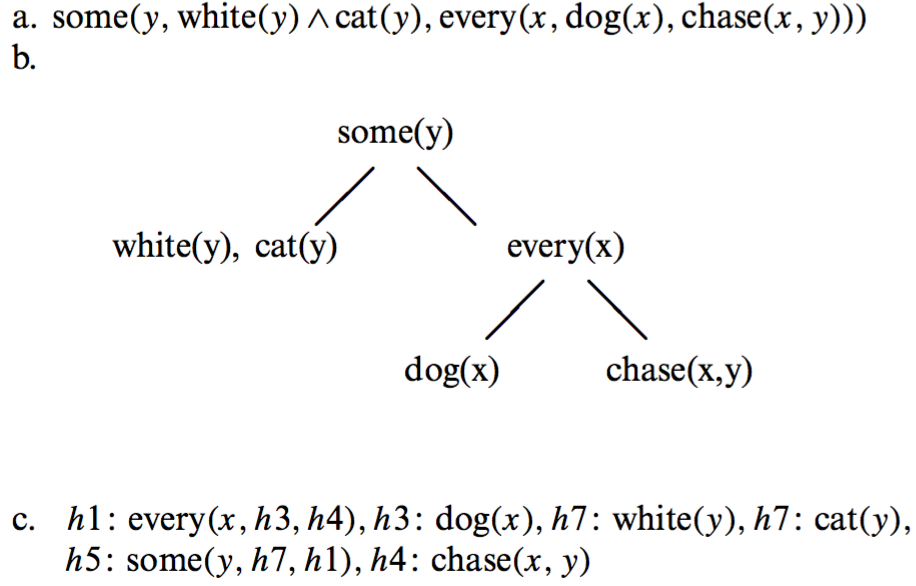
\includegraphics[height=4cm,width=6cm]{img/parse01.png}
            
            \column{0.5\textwidth}
            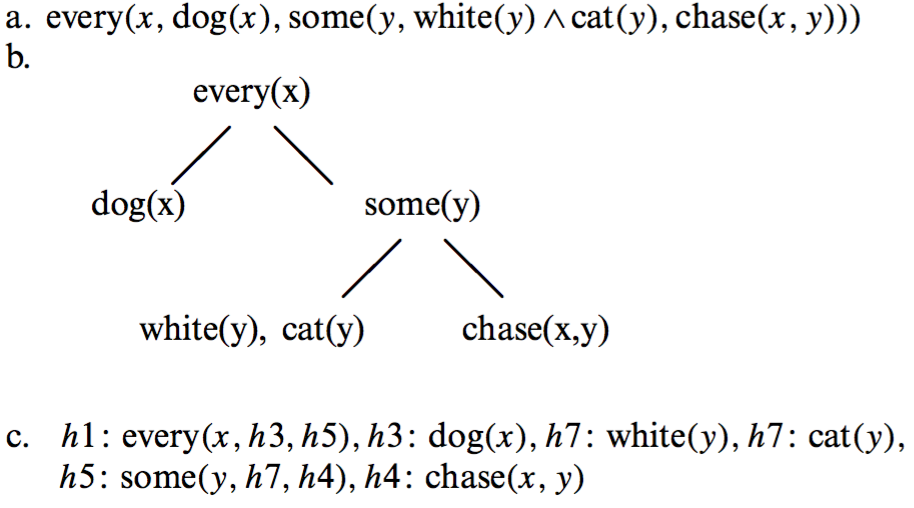
\includegraphics[height=4cm,width=6.3cm]{img/parse02.png}
        \end{columns}
    }

    \only<2>{
        \begin{columns}
            \column{0.7\textwidth}

            Leave some handles unspecified.

            \begin{itemize}

                \item Then specify it later: $h0 = h1, h3 = h5, h7 = h4$

                \item constraints, $h3 \neq h7$ to make it still a tree

                \item qeq constraint, $h0 =_q h5$ is a trival example

            \end{itemize}

            \column{0.3\textwidth}

            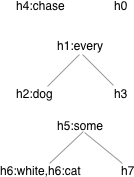
\includegraphics[height=4cm]{img/unresolved-parse.png}

        \end{columns}
    }

\end{frame}

\begin{frame}
    \frametitle{MRS formally in a whole}

    MRS is a quadruple \{GT, LT, R, C\}

    \begin{itemize}
        \item GT: global top. h0
        \item LT: local top. h1, h4, h5 (semantic of local phrase)
        \item R: relations. h1:every(x, h2, h3), h5:dog(y, h6, h7), h4:chase(x), etc.
        \item C: constraints. h0 qeq h4, etc.
    \end{itemize}
\end{frame}

\begin{frame}
    \frametitle{Highlights of MRS}

    \begin{itemize}
        \item We reify scopal relationships as handles
            so that syntactically the language looks first-order.
        \item Preserve \emph{underspecifiability}
    \end{itemize}
\end{frame}

\subsection{AMR}

\begin{frame}
    \frametitle{Abstract Meaning Representation (Banarescu, 2013)}

    AMR is an semantic representation that

    \begin{itemize}
        \item is rooted, directed and labeled graph
        \item is identical for different utterance
        \item uses variables for co-reference
        \item uses PropBank frame (analogous to roles in neo-Davidsonian)
        \item designs non-core relations out of PropBank
            (analogous to adjuncts in neo-Davidsonian)
    \end{itemize}

    Specification: https://github.com/amrisi/amr-guidelines/blob/master/amr.md

\end{frame}

\begin{frame}[fragile] % fragile is for verbatim
    \frametitle{An AMR Example}

    \emph{Brutus stabbed Caesar with a knife in the back in the agora and twisted it hard.}

    \begin{verbatim}
(s / stab
      :ARG0 (p / person :name (n / name :op1 "Brutus")
            :ARG0-of (t / twist
                  :ARG1 k
                  :manner (h / hard)))
      :ARG1 (p2 / person :name (n2 / name :op1 "Caesar"))
      :ARG2 (k / knife)
      :ARG3 (b / back)
      :location (a / agora))
    \end{verbatim}
\end{frame}

\begin{frame}[fragile]
    \frametitle{Event Frames Rise from Various POS}

    \begin{itemize}
        \item Verb \pause
        \item Noun

            \begin{examples}
            \emph{the destruction of the city by the God}
            \begin{verbatim} (d / destroy-01 :ARG0 (g / God) :ARG1 (c / city)) \end{verbatim}
            \end{examples}

            \begin{examples}
            \emph{the bond investor}
            \begin{verbatim} (p / person :ARG0-of (i / invest-01 :ARG1 (b / bond))) \end{verbatim}
            \end{examples}

            \only<2>{but \emph{professor} doesn't yield an event frame}

            \pause

        \item Adjective

            \begin{examples}
            \emph{the attractive spy}
            \begin{verbatim} (s / spy :ARG0-of (a / attract-01)) \end{verbatim}
            \end{examples}
    \end{itemize}
\end{frame}

\begin{frame}[fragile]
    \frametitle{Reification - Frame from Non-Core Relation}

    An adjunct for non-core relation in AMR must serve as a role for the relation,
    rather than for any object participating in that relation.

    \begin{examples}
    \emph{the marble in the jar}
    \begin{verbatim} (m / marble :location (j / jar)) \end{verbatim}

    \emph{the marble is not in the jar}
    \begin{verbatim} (b / be-located-at-91
    :ARG1 (m / marble) :ARG2 (j / jar) :polarity -) \end{verbatim}
    \end{examples}

    \begin{alertblock}{Semantic Error}
    \begin{verbatim} (m / marble :location (j / jar :polarity -)) \end{verbatim}
    which reads \emph{the marble is in the non-jar}
    \end{alertblock}
\end{frame}

\begin{frame}
    \frametitle{Other Language Phenomenons Defined in AMR}

    AMR defines approximately 100 relations for language phenomenons.

    \begin{itemize}
        \item negation and modals
        \item interrogation and wh-questions
        \item named entities
        \item location source, destination, path
        \item cause, concession, condition
        \item quantities, date, time
        \item link with wikipedia article :wiki ``Barack\_Obama''
        \item \dots
    \end{itemize}

\end{frame}

\begin{frame}
    \frametitle{AMR Data Overview}

    1. Annotated Corpus:

    \begin{itemize}
        \item \emph{The Little Prince}, 1274:145:143
        \item \emph{The Little Prince} Chinese Version, 1274:145:143
        \item Bio AMR Corpus from PubMed (cancer) articles, 5452:500:500
        \item LDC Corpus General Release 1.0 (June 2014), 13051 in all, \\
            a new general release is due in summer of 2016
    \end{itemize}

    2. Evaluation: smatch metric, comparison of two AMR

    3. SemEval-2017 Task 9: Parsing and Generation

    \begin{itemize}
        \item English Biomedical Data to AMR (SemEval-2016 Task 8)
        \item AMR to English Generation
    \end{itemize}

    4. A python parser: https://github.com/nschneid/amr-hackathon

\end{frame}
\begin{frame}
    \frametitle{Chinese AMR Corpus Example}

    \begin{center}
        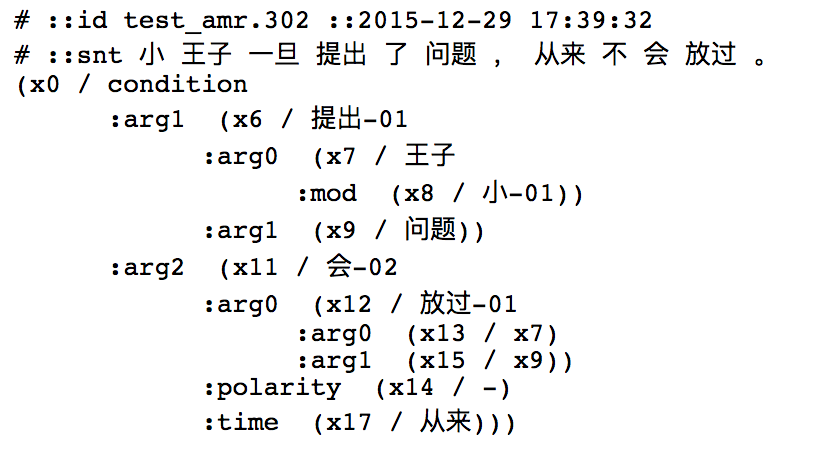
\includegraphics[height=7cm,width=12cm]{img/little-prince-chn-parse.png}
    \end{center}
\end{frame}

\begin{frame}
    \frametitle{AMR Editor}

    A simple web editor to build an AMR.

    \begin{center}
        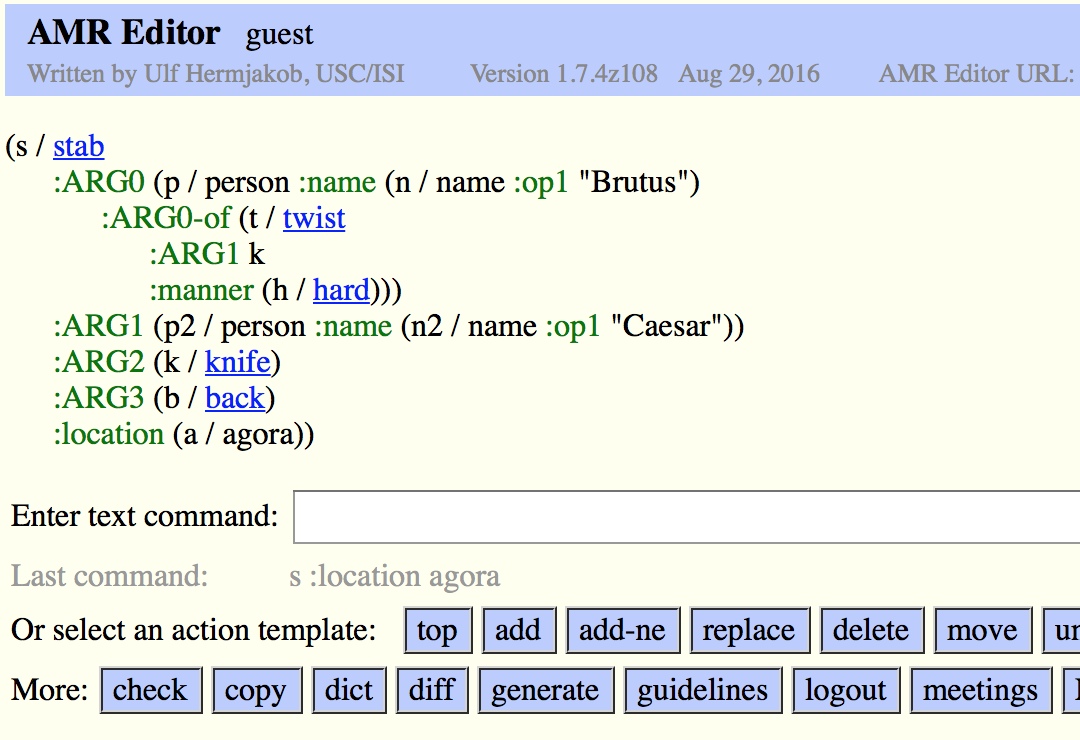
\includegraphics[height=6.7cm,width=9.8cm]{img/amr-editor.png}
    \end{center}
\end{frame}

\section{Parsing}

\begin{frame}
    empty
\end{frame}

\end{document}
